\section{Solução desenvolvida}\label{sec:solucao-desenvolvida}

\begin{figure*}[ht]
\centering
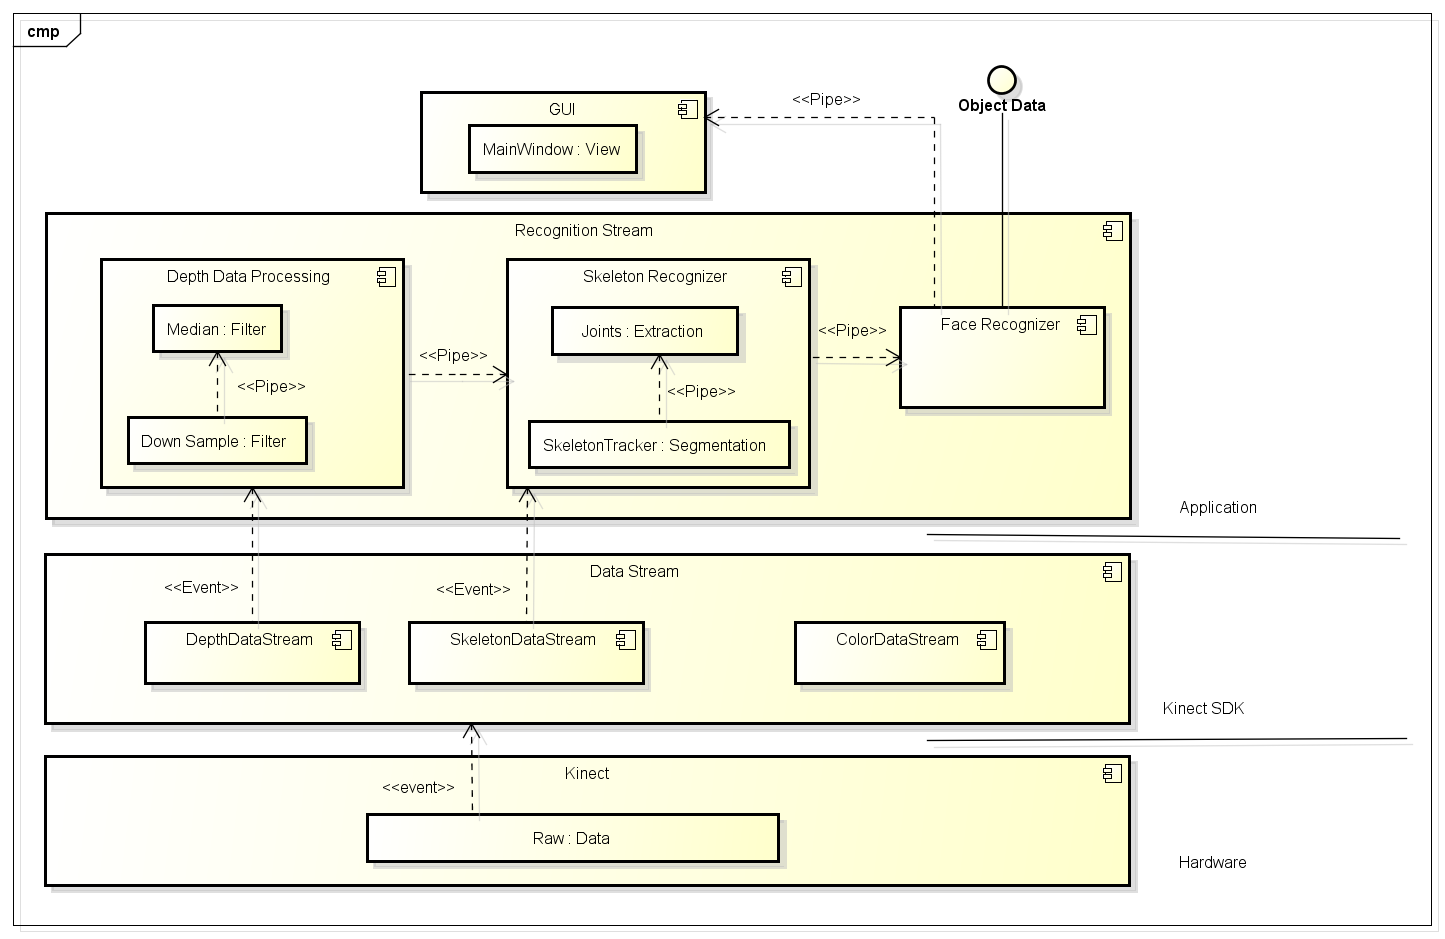
\includegraphics[width=1.0\textwidth]{images/Arquitetura_da_solucao.png}
\caption{Arquitetura da solução desenvolvida}
\label{fig:visao-geral}
\end{figure*}

Motivado pela demanda de serviços de identificação de pessoas e pelo fato de que as soluções para tal problema ainda permanecem em aberto, este trabalho propõe a utilização de mapas de profundidade. O mecanismo de identificação consiste em extrair esse mapa através do projetor infravermelho e do sensor monocromático, e analisar os dados obtidos, utilizando de filtros e algoritmos de segmentação. Por fim, é exibida graficamente uma visualização do mapa de profundidade gerado e, em caso de positivo, o(s) indivíduo(s) encontrado(s) na cena. É exibido também os dados que podem ser exportados para plataformas externas: a localização aproximada dos sujeitos no plano 3D (posições $X$, $Y$ e $Z$) e a distância em relação ao \textit{Kinect}. Nesta seção é discutida a solução desenvolvida.

\subsection{Arquitetura da solução}\label{sec:arqSol}
Para processar os dados de profundidade do sensor \textit{Kinect}, a aplicação executa o seguinte fluxo de dados:

\begin{enumerate}
    \item Habilitar o canal de fluxo de profundidade com o tipo de formato de imagem em profundidade; 
    \item Anexar o manipulador de eventos ao canal de fluxo; 
    \item Processar os quadros de profundidade de entrada; 
    \item Renderizar os quadros na UI.
\end{enumerate}

O \textit{Kinect} é o responsável por obter a visualização da cena de um ambiente interno. Como discutido na seção \ref{sec:trabalhos-relacionados}, o \textit{Kinect} é um sensor de movimento muito eficiente, extraindo com precisão objetos, pessoas e detalhes de uma cena. A \textit{Microsoft} provê para o \textit{Kinect} um Kit de desenvolvimento de software (\textit{Software Development Kit}, SDK). O sistema é composto por módulos adicionados à camada de aplicação, Sobre a camada do SDK. A Figura \ref{fig:visao-geral} apresenta uma visão geral da solução.

\subsubsection{Estilos arquiteturais}\label{sec:estilosArq}
A solução apresenta um estilo arquitetural híbrido, com características de três estilos arquiteturais básicos:

\begin{itemize}
\item Baseado em invocação implícita: \textit{Event Based}; 
\item Baseado em fluxo de dados: \textit{Pipe and Filter}; 
\item Em camadas: \textit{Virtual Machine}.
\end{itemize}

O estilo baseado em eventos (\textit{Event Based}) é um estilo arquitetônico baseado na invocação implícita que fornece uma interação indireta entre componentes acoplados de forma livre, facilitando a adaptação e melhorando a escalabilidade do sistema. Os componentes do tipo de evento (\textit{Depth}, \textit{color} e \textit{Infrared}.) comunicam-se apenas através de eventos transmitidos por um conector \textit{event}.
Este conector então retransmite os eventos para todos os componentes do tipo \textit{Observer} mostrando interesse no evento em questão (Nesse caso, o \textit{Recognition Stream}), melhorando assim a eficiência da distribuição de eventos.

\textit{Pipes} e Filtros (\textit{Pipe and Filter}) é um estilo arquitetural composto por uma cadeia de elementos de processamento, dispostos de forma tal que a saída de cada elemento é a entrada do próximo. O fluxo de dados se dá através de \textit{pipes} (canos) e os dados sofrem transformações quando processados nos filtros. Em outras palavras, os \textit{pipes} é que possibilitam o fluxo dos dados, e os filtros fazem o processamento dos mesmos, colocando-os nos \textit{pipes} antes que todos os dados de entrada sejam consumidos. Portanto, a nível de arquitetura, o processamento é mapeado em filtros e os \textit{pipes} agem como condutores de dados. O componente \textit{Recognition Stream} é composto por subcomponentes do tipo \textit{Filter} e a comunicação entre os mesmos se dá através dos conectores do tipo \textit{Pipe}. 

As arquiteturas de máquinas virtuais (\textit{Virtual Machines}) têm como objetivo alcançar a qualidade da portabilidade. Este estilo de arquitetural simula algumas funcionalidades que não são originais para o \textit{hardware} e/ou \textit{software} em que é implementado. O estilo é aplicado entre o \textit{Kinect (hardware)} e a aplicação desenvolvida, usando conectores do tipo \textit{Event} e \textit{Pipe} entre as camadas. Esse estilo arquitetônico reduz a complexidade, melhora a modularidade, reutilização e manutenção.
Conforme visto na figura \ref{fig:visao-geral}, o sistema possui as camadas:

\begin{itemize}
\item \textit{Kinect (hardware)};
\item \textit{Kinect} SDK; 
\item Aplicação; 
\end{itemize}

\subsubsection{Arquitetura do \textit{Kinect for Windows} SDK}\label{sec:kinectSDK}
O SDK fornece uma biblioteca e ferramentas de software sofisticadas para ajudar os desenvolvedores a usar a forma rica de entrada natural baseada no uso do \textit{Kinect}, que detecta e reage a eventos do mundo real. O \textit{Kinect} e a biblioteca de software interagem com aplicações, como mostrado na Figura \ref{fig:sdk_interact}. Os componentes do SDK são exibidos na figura \ref{fig:sdk_architecture_color} e incluem:

\begin{enumerate}
    \item \textit{Hardware Kinect} - Os componentes de \textit{hardware}, incluindo o sensor \textit{Kinect} e o \textit{hub} USB através dos quais o sensor \textit{Kinect} está conectado ao computador;
    \item \textit{Drivers Kinect} - Os \textit{drivers} do Windows para o \textit{Kinect}, que são instalados como parte do processo de configuração do SDK. Os \textit{drivers} do \textit{Kinect} suportam:
        \begin{itemize}
            \item A matriz de microfones como um dispositivo de áudio em modo \textit{kernel} que pode ser acessado  através das API de áudio padrão no \textit{Windows}; 
            \item Controles de transmissão de áudio e vídeo para transmissão de áudio e vídeo (cor, profundidade e esqueleto);
            \item Funções de enumeração de dispositivos que permitem que um aplicativo use mais de um \textit{Kinect}.	
        \end{itemize} 
    \item Componentes de Áudio e Vídeo:
        \begin{itemize}
            \item Interface de usuário natural do \textit{Kinect} para rastreamento de esqueleto, áudio e imagem em cores e profundidade. 
        \end{itemize}
    \item Objeto de mídia \textit{DirectX} (DMO) para formatação de feixes de microfone e localização de fonte de áudio;
    \item API padrão do \textit{Windows} - APIs de áudio, voz e mídia no \textit{Windows}, conforme descrito no SDK do \textit{Windows} e no \textit{Microsoft} \textit{Speech} SDK.
\end{enumerate}

\begin{figure}[ht]
\centering
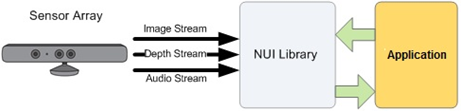
\includegraphics[width=0.48\textwidth]{images/sdk_interaction.png}
\caption{Interação de Hardware e Software com a Aplicação}
\label{fig:sdk_interact}
\end{figure}

\begin{figure*}[ht]
\centering
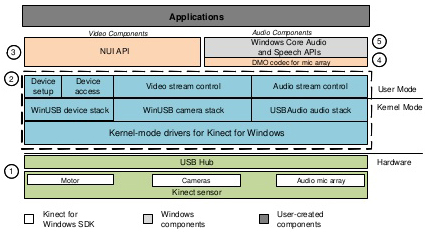
\includegraphics[width=0.7\textwidth]{images/sdk_architecture_color.png}
\caption{Arquitetura do SDK}
\label{fig:sdk_architecture_color}
\end{figure*}

\subsection{Componentes principais}\label{sec:componentes}

\subsubsection{\textit{Color Data Stream}}\label{sec:colorDataStream}
O \textit{Kinect} SDK fornece uma classe base abstrata \textit{ImageStream}. Essa classe é implementada tanto pelas classes de \textit{stream} de cores quanto de profundidade. Para a classe \textit{ColorImageStream}, o fluxo é realizado pelos seguintes passos: ativa o fluxo, captura o fluxo quadro a quadro no aplicativo e processa os quadros de imagens recebidas.

Quando o sensor está em execução, e o \textit{stream} RGB está habilitado, o sensor é inicializado  \textit{Kinect} para gerar um fluxo de imagens coloridas. A próxima etapa é informar ao sensor o que fazer quando for capturado um novo \textit{frame} de imagem. Para tal, é utilizado um manipulador de eventos que deve ser anexado ao canal do fluxo do sensor. O método \textit{ColorStream.Enable()} é um método sobrecarregado que por \textit{default} não recebe argumento, gerando uma resolução de  640x480 \textit{pixels} à 30Fps. Essa resolução \textit{default} é a utilizada nesse projeto. A classe \textit{KinectSensor} possui um evento \textit{ColorFrameReady}, que é invocado sempre que há novo quadro enviado pelo sensor. O manipulador de eventos possui dois argumentos: o primeiro é um remetente e o segundo um \textit{ColorImageFrameReadyEventArgs}.

\begin{minted}{csharp}
this.sensor = KinectSensor.KinectSensors.
  FirstOrDefault(sensorItem => 
  sensorItem.Status == 
  KinectStatus.Connected);
this.StartSensor();
this.sensor.ColorStream.Enable();
this.sensor.ColorFrameReady += 
  sensor_ColorFrameReady;
\end{minted}


Uma vez que o manipulador de eventos é chamado, significa que há um novo quadro que foi enviado pelo sensor e é hora de processá-lo. Os argumentos do evento para este manipulador de eventos expõem um método \textit{OpenColorImageFrame()} que retorna um \textit{frame} de imagem do tipo \textit{ColorImageFrame}. Com isso, o controle da aplicação se move para o Manipulador de eventos \textit{sensor\_ColorFrameReady}, responsável por designar os dados da câmera RGB para o devido  processamento do quadro de imagem no \textit{Skeleton Recognizer}. 

\subsubsection{\textit{Depth Data Stream}}\label{sec:depthDataStream}

Quando se trata do \textit{Kinect}, há apenas uma imagem, que é capturada pelo sensor de profundidade IR. Então, como funciona a triangulação estéreo? Na verdade, existem duas imagens em vez de uma. A segunda imagem é invisível - é um padrão do emissor IR, já definido com o laser IR. O laser IR não é modulado. Tudo o que o laser faz é projetar um padrão pseudo-aleatório de especificações no ambiente \textit{Kinect}. Essas duas imagens não são equivalentes, pois há alguma distância entre o emissor IR e o sensor de profundidade IR. Essas duas imagens são consideradas como correspondência para diferentes câmeras e permitem a aplicação de triangulação estéreo para calcular a profundidade como mostrado na imagem \ref{fig:trilatStereo}. Essa imagem demonstra como $x1$ e $x2$ são medidos usando a triangulação estéreo para um ponto $X$ na cena. O sensor \textit{Kinect} retorna dados brutos do \textit{frame} de profundidade em 13 bits. Esses bits fornecem a distância medida em milímetros.

\begin{figure}[!ht]
\centering
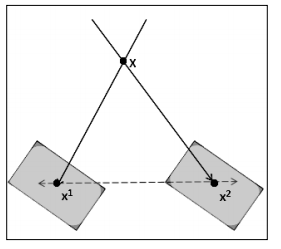
\includegraphics[width=0.4\textwidth]{images/trilateracao_estereo.png}
\caption{Trilateração estéreo para cálculo de profundidade.}
\label{fig:trilatStereo}
\end{figure}

o \textit{Depth Data Stream} lê os pontos na cena, processa os dados, de acordo com a equação \ref{eq:eq1} e envia a informação de profundidade a partir da qual eles foram refletidos, para o \textit{Recognition Stream}. Nele, é identificado o sensor \textit{Kinect} conectado e é ativado o canal do fluxo de profundidade.

A classe \textit{ImageStream} possui o método \textit{Enable()} sobrecarregado. Por padrão, o sensor permite o fluxo de profundidade com o formato de imagem de profundidade de resolução 640x480 \textit{pixels} e 30 \textit{frames} por segundo (\textit{Resolution640x480Fps30}).

Uma vez que o sensor é identificado e o fluxo de profundidade está habilitado, é anexado o manipulador de eventos \textit{DepthFrameReady} a um evento que é gerado cada vez que um novo \textit{frame} de profundidade está disponível:

\begin{minted}{csharp}
this.sensor = KinectSensor.KinectSensors[0];
this.sensor.DepthStream.Enable(
  DepthImageFormat.Resolution640x480Fps30);
sensor.DepthFrameReady +=
  new EventHandler
  <DepthImageFrameReadyEventArgs>
    (sensor_DepthFrameReady);
\end{minted}

\subsubsection{\textit{Skeleton Data Stream}}\label{sec:skeletonStream}
O sensor \textit{Kinect} retorna os dados brutos de profundidade, onde cada pixel contém um valor que representa a distância entre o sensor e o objeto. Os dados de profundidade fornecem possibilidades ilimitadas. Para essa solução, foi necessário obter controle usando o movimento do corpo. Primeiramente é necessário capturar a informação sobre os usuários que estão na frente do \textit{Kinect} e, a partir desse momento, identificar o mapeamento do esqueleto na imagem.

A informação dos \textit{frames} de esqueleto é representada por \textit{SkeletonStream}. A classe \textit{SkeletonStream} define as propriedades e métodos para trabalhar com dados de esqueleto e permite assumir o controle sobre todos os dados do esqueleto. Essa classe define também as propriedades para configurar o modo de rastreio para os \textit{Skeletons} e permite escolher o esqueleto certo para a aplicação usando o método \textit{AppChooseSkeletons()}. 

O recurso completo de rastreamento do esqueleto é construído com base em algoritmos de processamento de dados em profundidade, aprendizado de máquina interna e algoritmos de visão colorida (RGB). Usando o rastreamento do esqueleto, o sensor \textit{Kinect} pode rastrear o corpo humano com vários pontos de junção (\textit{joint points}). Usando o \textit{Kinect} é possível detectar até seis indivíduos e até 20 \textit{joints} para cada um deles. A Figura \ref{fig:human_joints} representa o esqueleto humano completo de frente, com os 20 pontos comuns que podem ser rastreados pelo \textit{Kinect}.

\begin{figure}[ht]
\centering
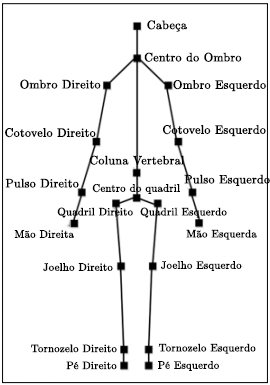
\includegraphics[width=0.4\textwidth]{images/human_joints.png}
\caption{\textit{Joints} capturados pelo \textit{Kinect}}
\label{fig:human_joints}
\end{figure}

\subsubsection{\textit{Depth Data Processing}: Filtros}\label{sec:depthDataProcessing}
O manipulador de eventos \textit{DepthFrameReady} é invocado com o argumento \textit{DepthImageFrameReadyEventArgs}, que possui o método \textit{OpenDepthImageFrame()} para retornar o quadro de imagem de profundidade atual enviado pelo sensor. O  método padrão para \textit{DepthFrameReady} é o \textit{SensorDepthFrameReady}. Nesse método, é recuperado o quadro de imagem em profundidade, usando o método \textit{OpenDepthImageFrame()}, o qual retorna os dados de profundidade brutos do sensor. \textit{PixelData} cria o tamanho do \textit{buffer} para o quadro de imagem de profundidade de entrada.
O \textit{frame} de profundidade possui propriedades semelhantes que copiam os dados de \textit{pixels} para o \textit{buffer} recém-criado. \textit{CopyPixelDataTo()} é usado para copiar o \textit{array} de bytes de dados de \textit{pixels} do quadro de imagem atualmente recebido para o \textit{buffer}. Antes de copiar os dados de \textit{pixels}, primeiro é calculado o tamanho do \textit{buffer} usando a propriedade \textit{PixelDataLength} e, em seguida, é copiada a mesma imagem do \textit{array} de bytes como \textit{DepthImageFrame}. Como o quadro bruto de imagem de profundidade é uma imagem em escala de cinza de 16 \textit{bits}, \textit{PixelFormats} é especificado  como \textit{Gray16} ao criar a fonte de \textit{bitmap} para o controle de imagem em profundidade.

\paragraph{\textit{DownSampleFilter}}\label{sec:DSfilter}
 Na imagem de profundidade gerada pelo \textit{Kinect}, todos os pontos que o sensor não consegue medir a profundidade são deslocados para 0 no \textit{array} de saída. Considerando  como um tipo de ruído, Para evitar sua interferência, é necessário recuperar seu verdadeiro valor de profundidade. Supondo que o espaço seja contínuo, o mais provável é que o ponto faltante tenha um valor de profundidade semelhante aos seus vizinhos. Com esta suposição, todos os 0 \textit{pixels} são considerados como vagos e precisam ser preenchidos. É utilizado então o algoritmo de interpolação vizinho mais próximo para preencher esses \textit{pixels} e obter uma matriz de profundidade que tenha valores significativos em todos os \textit{pixels}. Em seguida, é utilizado o filtro mediano com uma janela 4 x 4 na matriz de profundidade para tornar os dados suaves.

\paragraph{\textit{Median Filter}}\label{sec:Mfilter}
O filtro mediano é uma técnica de filtragem digital não-linear, usada frequentemente para remover o ruído de uma imagem ou sinal. Essa redução de ruído é um passo de pré-processamento típico para melhorar os resultados do processamento posterior (segmentação da uma imagem). A filtragem média é amplamente utilizada no processamento de imagens digitais porque, sob certas condições, preserva bordas ao mesmo tempo que remove o ruído. A ideia principal do filtro mediano é percorrer a entrada do sinal por entrada, substituindo cada entrada pela mediana das entradas vizinhas. O padrão de vizinhos é chamado de "janela", que desliza, entrada por entrada, em todo o sinal. usando um tamanho de janela de três com uma entrada imediatamente anterior e seguindo cada entrada, um filtro mediano é aplicado ao  sinal, como exemplificado, para um conjunto de \textit{pixesls} $x = [2\,80\, 6 \,3]$:

\begin{align*}
x = [2\,\, 80\,\, 6 \,3]\MoveEqLeft[23]\\
y[1] = Mediana[2\,\, 2\,\, 80] = 2\MoveEqLeft[16.7]\\
y[2] = Mediana[2\,\, 80\,\, 6] = Mediana[2\,\, 6\,\, 80] = 6\MoveEqLeft[8]\\
y[3] = Mediana[80\,\, 6\,\, 3] = Mediana[3\,\, 6\,\, 80] = 6\MoveEqLeft[8]\\
y[4] = Mediana[6\,\, 3\,\, 3] = Mediana[3\,\, 3\,\, 6] = 3\MoveEqLeft[9]\\
y = [2\,\, 6\,\, 6\,\, 3]\MoveEqLeft[23].
\end{align*}

Finalmente, é criado o objeto \textit{BitmapSource} e atribuído ao controle de imagem \textit{depthImageControl}, que está definido no arquivo XAML para exibir os dados do fluxo.

\subsubsection{\textit{SkeletonRecognizer}: Segmentação}\label{sec:skeleton}

Neste componente, o fluxo de processamento obtém imagem segmentada em profundidade, usando o mapa de profundidade, já processado pelos filtros. Remove pequenas \textit{blobs}. Obtém posições candidatas para a cabeça e a parte superior do corpo utilizando o detector da parte superior do corpo. Corrige os pontos de cabeça, pescoço e ombro usando os retângulos delimitadores obtidos no passo anterior. Calcula a Transformação de Distância Estendida para a imagem de profundidade segmentada. Inicia uma busca angular para os melhores valores em torno das articulações do ombro. Retorna um \textit{array} com as posições dos \textit{joints}. Para esta solução, são utilizados apenas os \textit{joints} da região superior do corpo humano, evitando assim um processamento exaustivo com \textit{joints} desnecessários.

\paragraph{\textit{Skeleton tracker}}\label{sec:SkeletonTracker}
A classe \textit{SkeletonTracker} não é responsável apenas pelo rastreamento das articulações, lendo as informações de uma pessoa. Além disso, ele rastreia o movimento completo do corpo. O reconhecimento de pose humano em tempo real é difícil e desafiador devido às diferentes poses do corpo (uma única parte do corpo pode se mover em diferentes direções e maneiras), tamanhos (tamanhos de humanos variam), roupas do usuário, alturas (humano pode ser alto, baixo, médio), e assim por diante.

Para superar tais problemas e rastrear diferentes articulações independentemente da pose do corpo, o \textit{Kinect} usa um \textit{pipeline} de renderização que correlaciona os dados recebidos (dados de profundidade bruta do sensor) com dados treinados por amostra. O algoritmo de reconhecimento de pose humano usou vários modelos base de personagens, variando diferentes alturas, tamanhos, roupas e vários outros fatores. Os dados aprendidos da máquina foram coletados dos personagens. Os dados aprendidos da máquina são rotulados como partes individuais do corpo e combinados com os dados de profundidade de entrada para identificar a parte do corpo ao qual pertence. O pipeline de renderização processa os dados em várias etapas para rastrear as partes do corpo humano a partir de dados de profundidade.

As posições dos \textit{joints} são medidas por três coordenadas ($X, Y$ e $Z$), onde $X$ e $Y$ definem a posição do \textit{joint} e $Z$ representa a distância ao sensor. Para obter as coordenadas adequadas, o sensor calcula as três visualizações da mesma imagem: vista frontal, vista esquerda e vista superior, pelo qual o sensor define a proposta do corpo 3D. nesta classe, o fluxo de processamento  utiliza os dados de profundidade e combina com os dados da floresta de decisão e gera os segmentos do corpo. Uma vez que todas as partes são identificadas com base nos dados rotulados, o sensor identifica as articulações do corpo. O sensor calcula a vista 3D a partir da parte superior, frente e esquerda das juntas propostas. Então, o sensor começa a rastrear o esqueleto humano e o movimento do corpo com base nos pontos comuns propostos e na visão 3D.

O SDK do \textit{Kinect} fornece um conjunto de API's que facilitam a manipulação de \textit{joints}. Cada \textit{joint} é identificado pelo seu nome (cabeça, ombros, cotovelos, pulsos, braços, coluna, quadris, joelhos, tornozelos, etc.) e o estado do rastreamento, determinado por \textit{Tracked, Not Tracked,} ou \textit{Inferred}. Visando uma economia de recurso computacional, foram utilizados apenas dez desses \textit{joints}, representados na Figura  \ref{fig:human_joints2} .

\begin{figure}[ht]
\centering
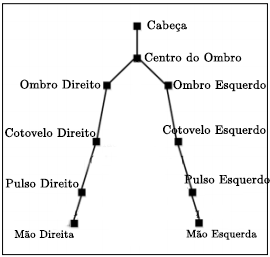
\includegraphics[width=0.4\textwidth]{images/human_joints_2.png}
\caption{\textit{Joints} superiores utilizados.}
\label{fig:human_joints2}
\end{figure}

O fluxo de processo para capturar dados de esqueleto é o mesmo que o usado para os fluxos de dados de cor e profundidade. os dados podem ser capturados usando o modelo de evento ou o modelo de \textit{polling}. O modelo utilizado na solução é o modelo de evento.  O objeto \textit{KinectSensor} tem um evento chamado \textit{SkeletonFrameReady}, que dispara cada vez que novos dados de esqueleto se tornam disponíveis no sensor. Cada quadro de \textit{SkeletonStream} produz uma coleção de objetos de esqueleto. Cada objeto de esqueleto contém os dados para seus pontos de junção, que estão envolvidos dentro do objeto \textit{JointCollection}. Cada articulação possui seu próprio tipo de modo de rastreamento e informações adicionais para representar as posições.

Sempre que uma nova estrutura de esqueleto é enviada pelos sensores, o método \textit{sensor\_SkeletonFrameReady()} é invocado já que está registrado no evento \textit{SkeletonFrameReady}. O método é invocado passando um argumento do tipo \textit{SkeletonFrameReadyEventArgs}. O argumento de evento tem um método chamado \textit{OpenSkeletonFrame()} que lê o objeto \textit{SkeletonFrame} atual do sensor. O objeto \textit{SkeletonFrame} é enviado então para o método \textit{PrintTrackedCoordinates}, responsável por calcular a distância entre o sujeito e o \textit{Kinect}. O método \textit{PrintTrackedCoordinates} obtém as coordenadas $X$, $Y$, e $Z$ dos dez \textit{joints} observáveis, calcula a distância, para cada um deles, e finalmente, calcula a média entre essas distâncias. O cálculo da distância leva em conta a distancia entre dois pontos no mapa: A (câmera do \textit{kinect}) e B (Pessoa) é obtida através da Fórmula \ref{eq:distancia1}:

\begin{align}
    d_{AB} &= \sqrt[]{{(X_{B} - X_{A})}^2 + {(Y_{B} - Y_{A})}^2 + {(Z_{B} - Z_{A})}^2}
    \label{eq:distancia1}
\end{align}

Que é derivada do teorema de Pitágoras e pode ser aplicado pra $n$ planos:

\begin{align}
    \sqrt[]{\sum_{i=1}^{n}{(i_{B} - i_{A})}^2}
    \label{eq:pitagoras}
\end{align}


Considerando o ponto inicial A (\textit{Kinect}) como coordenadas $(0,0,0)$, e aplicando esses valores sobre a Fórmula   \ref{eq:distancia1} temos então:
\begin{align}
    d_{AB} &= \sqrt[]{{X_{B}}^2 + {Y_{B}}^2 + {Z_{B}}^2} 
    \label{eq:distanciaFinal}
\end{align}


Aplicando a Fórmula na solução, temos, com arredondamento de três casas decimais:
\begin{minted}{csharp}
private double GetDistance
(SkeletonPoint point)
{
  return Math.Round(
    Math.Sqrt(
      Math.Pow(point.X, 2) +
      Math.Pow(point.Y, 2) +
      Math.Pow(point.Z, 2)
    ), 
  3);
}
\end{minted}

Finalizado o processo, o \textit{PrintTrackedData} imprime no console as informações de distância, coordenadas e índice identificador de cada sujeito detectado na cena, também com arrendondamento de tres casas decimais.
\begin{minted}{csharp}
private void PrintTrackedData
(Skeleton skeletonOfInterest)
{
  SkeletonPoint currentPosition = 
    skeletonOfInterest.Position;
  int index = skeletonOfInterest.
    TrackingId;
  String pattern = "0.000";
  String distance = GetDistance
    (currentPosition).ToString(pattern);
  String x = Math.Round(currentPosition.X,
    3).ToString(pattern);
  String y = Math.Round(currentPosition.Y,
    3).ToString(pattern);
  String z = Math.Round(currentPosition.Z,
    3).ToString(pattern);
  Debug.WriteLine(string.Format(
    "[Person ID: {0}]" +
    "[Distance: {1} m][Coordinates:" + 
    "  [X: {2}], [Y: {3}], [Z: {4}]" + 
    "]",
     index, distance, x, y, z));
}
\end{minted}

\subsubsection{Face Recognition}\label{sec:depthDataRecognition}

A classe de rastreamento de rostos \textit{FaceRecognizer} detecta e rastreia as posições e orientações dos rostos e também pode animar em tempo real as posições das sobrancelhas e a forma da boca. O rastreamento facial pode ser usado em vários locais, como o reconhecimento de expressões faciais, a interação Interface de usuário natural \textit{(Natural user interface} - NUI) com o rosto, e tarefas relacionadas ao rosto. Na aplicação desenvolvida, o rastreamento de rostos é utilizado apenas para visualização na interface gráfica, uma vez que as informações de interesse (distância e coordenadas) dos sujeitos na cena já foram obtidos após os processos de filtro e segmentação. A classe \textit{FaceTrackFrame} é o núcleo do sistema de detecção de faces, que representa o rosto para cada \textit{frame}. Através dela, é possível obter informações do posicionamento e do formato do rosto. O mecanismo analisa os dados de entrada, deduz a pose da cabeça e as expressões faciais e disponibiliza essa informação em tempo real, para a interface gráfica da aplicação.

O \textit{FaceTracking} usa o sistema de coordenadas para produzir seus resultados de rastreamento 3D. A origem está localizada no centro óptico da câmera (sensor), o eixo Z está apontando para o usuário, e o eixo Y está apontando para cima. As unidades de medida são metros, para translação e graus para ângulos de rotação.


\begin{figure}[ht]
\centering
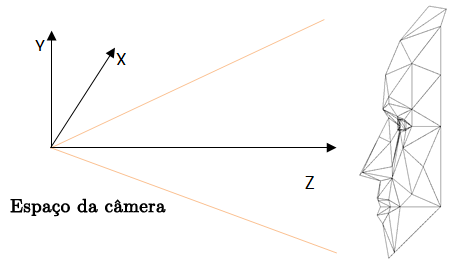
\includegraphics[width=0.4\textwidth]{images/3dface.png}
\caption{A máscara 3D calculada sobre o rosto do usuário (no quadro de coordenadas da câmera).}
\label{fig:3dfaces}
\end{figure}

O método \textit{DrawFaceModel}, descrito no Apêncice \ref{sec:apendiceA} é o responsável por fazer a plotagem dos dados da face. Esse método é responsável por criar e exibir uma malha poligonal 3D para cada face reconhecida. A nivel de diferenciação, para cada ser observável, uma cor do \textit{Array SolidColorBrush[] colors} é utilizada.


\subsubsection{Main Window (GUI)}\label{sec:mainWindow}

A classe \textit{MainWindow} contém a funcionalidade genérica do software. Ela contém um conjunto de variáveis globais para a funcionalidade adequada do código e métodos para as funções primárias do sistema. Quando o software é iniciado, ele executa o método \textit{MainWindow()} que inicializa os componentes da \textit{GUI}. Quando o método \textit{MainWindow()} é concluído, o \textit{MainWindowLoaded()} é executado, localizando o sensor \textit{Kinect} e instancia-o como um objeto, alocando as imagens de profundidade e a grade de reconhecimento facial na \textit{GUI}.

O método \textit{FacialRecognition()} é um manipulador de eventos que é acionado sempre que há uma nova imagem captada pelo \textit{Stream} do \textit{Kinect}. A imagem capturada pelo \textit{Kinect} é originalmente armazenada como uma imagem de \textit{bitmap}. Uma vez que isso ocorre, o método envia a imagem ao \textit{RecognitionStream} para executar os algoritmos de detecção, que em caso positivo, retorna os dados para serem exibidos em tela.

O método \textit{SkeletonTracking()} é outro manipulador de eventos que é executado sempre que o \textit{SkeletonStream} gera um novo \textit{SkeletonFrame}. O \textit{SkeletonStream} é uma abstração que determina onde cada pessoa está localizada no alcance do \textit{Kinect}. Cada \textit{SkeletonFrame} gerado pelo \textit{SkeletonStream} consiste em uma matriz de objetos de esqueleto, que por sua vez contém coordenadas tridimensionais para cada conjunto reconhecido pelo \textit{Kinect}, além da distância em relação ao \textit{kinect}. A matriz \textit{SkeletonFrame} não garante que o primeiro Esqueleto esteja localizado no índice zero da matriz, o segundo no índice um da matriz e assim por diante. Então um método percorre a matriz e determina quais esqueletos são realmente válidos antes de usá-los.

O método \textit{KinectSensorOnAllFramesReady()} é um manipulador de eventos que é acionado sempre que houver uma nova estrutura de dados da detecção de esqueleto ou de imagem de profundidade capturada pelo bloco de \textit{Stream}. Este evento é uma versão combinadas dos métodos \textit{FacialRecognition()} e \textit{SkeletonTracking()}.